% Byte range diagram: incremental update before/after signing (Chapter 13)
\documentclass[border=10pt]{standalone}
\usepackage{tikz}
\usetikzlibrary{positioning, decorations.pathreplacing, calc}
\usepackage{fontspec}
\setmainfont{Noto Serif}
\setsansfont{Noto Sans}
\setmonofont{DejaVu Sans Mono}[Scale=0.85]
\usepackage{xcolor}
\definecolor{original}{HTML}{e3f2fd}
\definecolor{appended}{HTML}{c8e6c9}
\definecolor{accent}{HTML}{0f3460}

\begin{document}
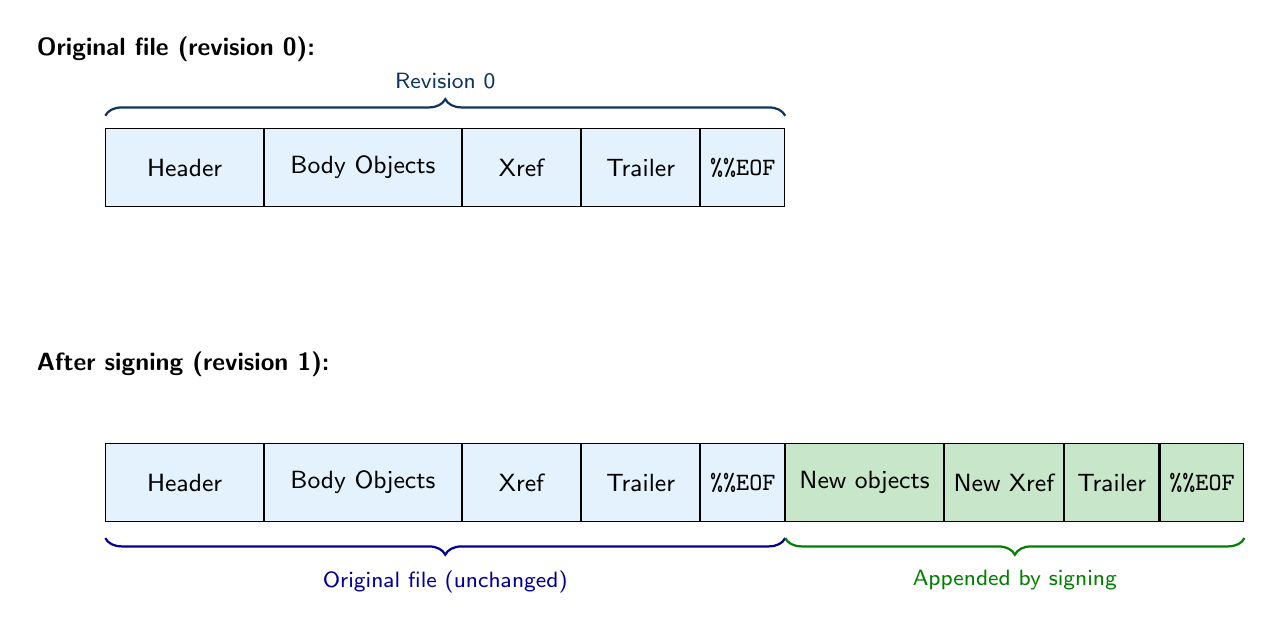
\begin{tikzpicture}[
    block/.style={draw, minimum height=1cm, text centered, font=\sffamily\small},
    brace/.style={decorate, decoration={brace, amplitude=6pt, mirror}},
    braceup/.style={decorate, decoration={brace, amplitude=6pt}},
]

% Row 1: Original file
\node[font=\sffamily\bfseries\small, anchor=west] at (0, 1.5) {Original file (revision 0):};

\node[block, fill=original, minimum width=2cm] (o1) at (2, 0) {Header};
\node[block, fill=original, minimum width=2.5cm, right=0pt of o1] (o2) {Body Objects};
\node[block, fill=original, minimum width=1.5cm, right=0pt of o2] (o3) {Xref};
\node[block, fill=original, minimum width=1.5cm, right=0pt of o3] (o4) {Trailer};
\node[block, fill=original, minimum width=1cm, right=0pt of o4] (o5) {\texttt{\%\%EOF}};

\draw[braceup, thick, accent] ($(o1.north west) + (0,0.15)$) -- node[above=6pt, font=\sffamily\footnotesize, text=accent] {Revision 0} ($(o5.north east) + (0,0.15)$);

% Row 2: After signing
\node[font=\sffamily\bfseries\small, anchor=west] at (0, -2.5) {After signing (revision 1):};

\node[block, fill=original, minimum width=2cm] (a1) at (2, -4) {Header};
\node[block, fill=original, minimum width=2.5cm, right=0pt of a1] (a2) {Body Objects};
\node[block, fill=original, minimum width=1.5cm, right=0pt of a2] (a3) {Xref};
\node[block, fill=original, minimum width=1.5cm, right=0pt of a3] (a4) {Trailer};
\node[block, fill=original, minimum width=1cm, right=0pt of a4] (a5) {\texttt{\%\%EOF}};
\node[block, fill=appended, minimum width=2cm, right=0pt of a5] (a6) {New objects};
\node[block, fill=appended, minimum width=1.2cm, right=0pt of a6] (a7) {New Xref};
\node[block, fill=appended, minimum width=1.2cm, right=0pt of a7] (a8) {Trailer};
\node[block, fill=appended, minimum width=0.8cm, right=0pt of a8] (a9) {\texttt{\%\%EOF}};

\draw[brace, thick, blue!60!black] ($(a1.south west) + (0,-0.2)$) -- node[below=8pt, font=\sffamily\footnotesize, text=blue!60!black] {Original file (unchanged)} ($(a5.south east) + (0,-0.2)$);
\draw[brace, thick, green!50!black] ($(a6.south west) + (0,-0.2)$) -- node[below=8pt, font=\sffamily\footnotesize, text=green!50!black] {Appended by signing} ($(a9.south east) + (0,-0.2)$);

\end{tikzpicture}
\end{document}
